\documentclass[10pt,a4paper]{article}
\usepackage[margin=1.5cm]{geometry}
\usepackage[utf8]{inputenc}
\usepackage[english]{babel}
\usepackage{amsmath}
\usepackage{amsfonts}
\usepackage{amssymb}
\usepackage{graphicx}
\usepackage{epstopdf}
\usepackage{epsfig}
\usepackage[font=footnotesize]{subfig}
\usepackage{hyperref}
\usepackage{eufrak}
\usepackage{xcolor}
\graphicspath{ {./img/} }



\author{generated by MDSip-test tools}
\title{MDSip throughput tests report}




\begin{document}

\maketitle

The MDSplus framework is a widespread tool used within many plasma physics laboratories.
It has been designed for acquisition and storage of complex scientific data but it is also able to remotely an easily access archived data along a network.
The remote data access is assigned to a particular specific MDSPlus  client/server component called \emph{mdsip} that is the subject of the present analysis report.
Due to the expected growing internationalization of big fusion experiments MDSplus is going to be applied to share experimental data between long distance endpoints.
For this reason the need of a network optimization was foreseen as an important concern for these applications.
A specific \emph{mdsip} test campaign was started at the beginning of this year and in this document we report the initial network performance results related to the Internet link between Italy and Japan.

\section{Software setup}

A specific software package has been required to perform the throughput tests for \emph{mdsip}.
Such software has been developed using the MDSplus framework C++ object libraries and it has been publicly released (download is available via github at: \url{https://github.com/MDSplus/MDSip-tests}).

It aims at providing a flexible layer to perform different timing tests writing data on the remote MDSplus \emph{mdsip} server. 
The tests are focused on finding an optimal data segment size and the connection characteristics of the internet long-distance network path between participants endpoint.
The overall testing software is organized in two layers: a general library and some testing recipes binaries. 
The library provides some utility classes that were implemented to obtain an easy~to~use environment.  

% sistemare %

The test chain of each recipe is always using three main types: the Content, the Channel, and the TestConnection. 
The Content represents the content of the segment to be sent, it can be a function generator (sine or white/gaussian noise for now) or a parse tree reader (captured connecting to a local \emph{mdsip} server). 
The Channel is responsible to actually send the segment to the endpoint, two channel flavours can be chosen using Distribute Client (DC) or Thin Client (TC) connections. Finally the TestConnection collects all different contents and channels and starts the connection itself. Two versions of TestConnection are implemented to manage parallel channels, the TestConnectionMT uses multiple threads (one per channel) and the TestConnectionMP uses different forked process.
~
Time and speed histograms are instanced by the TestConnection one per added channels, they account the timing of each put segment operation performed by the channel. This feature was introduced to produce a speed information that does not comprehend the time to generate the signal and the tree opening and closing operations. 
Furthermore the speed is computed using the actual size of the sent data, so all the results that will follow are representing the equivalent speed in KB per seconds of transmitted Float32 data. 
Obviously we expect this data to be higher bounded by the actual network capacity, a comparison test can be done with the results of a widely used tool called iperf.

\section{Network characterization}

The testing software has been installed on a 10Gbps connected machine \emph{test10g.nifs.ac.jp} (CentOS release 6.6 Final) located at NIFS\footnote{National Institute for Fusion Science, Toki City, Japan}, equipped with a Network Interface Controller Intel X520-DA2 directly connected through a 10GBASE-SR optical link to the SINET uplink router.
Such server acts as target endpoint and has been properly configured in order to allow connections coming from the client computer \emph{eprobe.igi.cnr.it} (CentOS release 6.5 Final) server at RFX\footnote{Reversed Field Experiment, Padova, Italy} equipped with a 1 Gbit/s NIC and directly connected by means of a 1000~BaseLX optical fiber link to the GARR uplink router.
~
Both computers were installed with the latest available version of MDSplus in alpha release keeping up to date with the latest features and changes of the framework.
All the software involved has been compiled using gcc 4.4.7 compiler.

A simple route tracing reveals 14 hops between the end points with a total connection RTT of 300~ms. 
The traceroute command outputs follow in Figure~(\ref{fig:hops}) where it can be seen that the connection is handled within the GEANT network, from the italian GARR consortium to SINET in Japan.

\begin{figure}[htbp!]
\begin{minipage}{.5\textwidth}
{ \tiny \begin{verbatim}
# traceroute -T -p 22 133.75.254.101
traceroute to 133.75.254.101 (133.75.254.101), 30 hops max, 40 byte packets
 1  150.178.3.1 (150.178.3.1)  5.392 ms  5.341 ms  5.338 ms
 2  192.168.4.10 (192.168.4.10)  0.558 ms  0.876 ms  1.167 ms
 3  150.178.101.1 (150.178.101.1)  5.969 ms  6.115 ms  6.314 ms
 4  ru-cnrpd-rx1-pd2.pd2.garr.net (193.206.132.193)  5.675 ms  5.666 ms  5.652 ms
 5  rx1-pd2-rx1-bo1.bo1.garr.net (90.147.80.13)  15.255 ms  19.800 ms  15.233 ms
 6  rx1-bo1-rx1-mi1.mi1.garr.net (90.147.80.109)  16.223 ms  15.507 ms  15.583 ms
 7  rx1-mi1-rx1-mi2.mi2.garr.net (90.147.80.82)  13.046 ms  12.679 ms  12.599 ms
 8  garr.mx1.mil2.it.geant.net (62.40.125.180)  15.282 ms  13.119 ms  15.129 ms
 9  ae6.mx1.gen.ch.geant.net (62.40.98.112)  25.093 ms  23.749 ms  22.501 ms
10  sinet.mx1.gen.ch.geant.net (62.40.125.242)  144.219 ms  139.506 ms  136.570 ms
11  osaka-dc-gm1-xe4-1-1-vlan10.s4.sinet.ad.jp (150.99.2.105)  297.703 ms  298.599 ms  297.671 ms
12  osaka-dc-rm-ae3-vlan10.s4.sinet.ad.jp (150.99.2.57)  297.714 ms  297.568 ms  297.532 ms
13  nagoya-dc-rm-ae1-vlan10.s4.sinet.ad.jp (150.99.2.33)  301.580 ms  304.463 ms  302.028 ms
14  nifs-Lan1.sinet.ad.jp (150.99.197.146)  306.228 ms  308.388 ms  308.317 ms
15  test10g.nifs.ac.jp (133.75.254.101)  310.353 ms  309.973 ms  310.855 ms
\end{verbatim} }
\end{minipage} 
~
\begin{minipage}{.5\textwidth}
{ \tiny \begin{verbatim}
# traceroute -T -p 22 rfxssh.igi.cnr.it
traceroute to rfxssh.igi.cnr.it (150.178.3.150), 30 hops max, 60 byte packets
 1  133.75.254.251 (133.75.254.251)  0.639 ms  0.653 ms  0.732 ms
 2  nagoya-dc-RM-AE2-102.s4.sinet.ad.jp (150.99.197.145)  8.233 ms 8.176 ms  8.186 ms
 3  osaka-dc-rm-ae0-vlan10.s4.sinet.ad.jp (150.99.2.34)  13.516 ms 13.513 ms  13.442 ms
 4  osaka-dc-gm1-ae0-vlan10.s4.sinet.ad.jp (150.99.2.58)  13.563 ms 13.498 ms  13.556 ms
 5  wdc-dc-gm1-xe1-0-0-vlan10.s4.sinet.ad.jp (150.99.2.106)  199.495 ms  199.471 ms  199.485 ms
 6  sinet-gw.mx1.gen.ch.geant.net (62.40.125.241)  295.572 ms  293.882 ms  293.864 ms
 7  ae1.mx1.mil2.it.geant.net (62.40.98.113)  300.171 ms  300.100 ms 300.139 ms
 8  garr-gw.mx1.mil2.it.geant.net (62.40.125.181)  300.118 ms  300.122 ms  300.103 ms
 9  rx1-mi2-rx1-mi1.mi1.garr.net (90.147.80.81)  308.143 ms  308.147 ms  307.619 ms
10  rx1-mi1-rx1-bo1.bo1.garr.net (90.147.80.110)  304.853 ms  310.155 ms  304.867 ms
11  rx1-bo1-rx1-pd2.pd2.garr.net (90.147.80.14)  308.429 ms  310.645 ms  308.504 ms
12  rx1-pd2-ru-cnrpd.pd2.garr.net (193.206.132.194)  308.791 ms  310.125 ms  307.811 ms
13  150.178.101.2 (150.178.101.2)  309.229 ms  310.109 ms  311.320 ms
\end{verbatim} }
\end{minipage} 
\caption{Traceroute output between ra22.igi.crn.it(RFX) and test10g.nifs.ac.jp(NIFS) }  
\label{fig:hops}
\end{figure}

The network link has been further characterized using the iperf tool in TCP and UDP. 
At the RFX side Garr declares a backbone connection of 1~Gbps so we used this specification and the measured RTT value to properly tune the TCP stack.
The send and receive buffers of IPv4 sockets were adjusted to 32~MB assuming no congestion and no packet loss in the network. %according to RFC3155
A plot of the obtained bandwidth in TCP using different Window sizes is plotted in Figure~(\ref{fig:iperf_a}).

Iperf UDP tests have also been performed between two SINET nodes and show that the effective UDP throughput in Japan is about 3~Gbps.
The maximum UDP bandwidth of RFX consortium is instead limited at 1~Gbps from GARR, as it can be seen in Figure~(\ref{fig:iperf_b}) where iperf test is reported with a maximum bandwidth of 800~Mbps
\footnote{iperf seems to underestimate the real bandwidth in UDP sessions with high transmission rates due to lack of cpu resources}.
Therefore the maximum transfer speeds are capped by the RFX up-link limit and we have no chance to get a true internet connection performance measure, and it will not be presented here.
As a consequence the role of this document will be to report a comparison between the maximum network bandwidth observed between this two nodes and the actual transfer rate achieved by \emph{mdsip} connection.

\begin{figure}[htbp!]
\centerline{
\subfloat[]{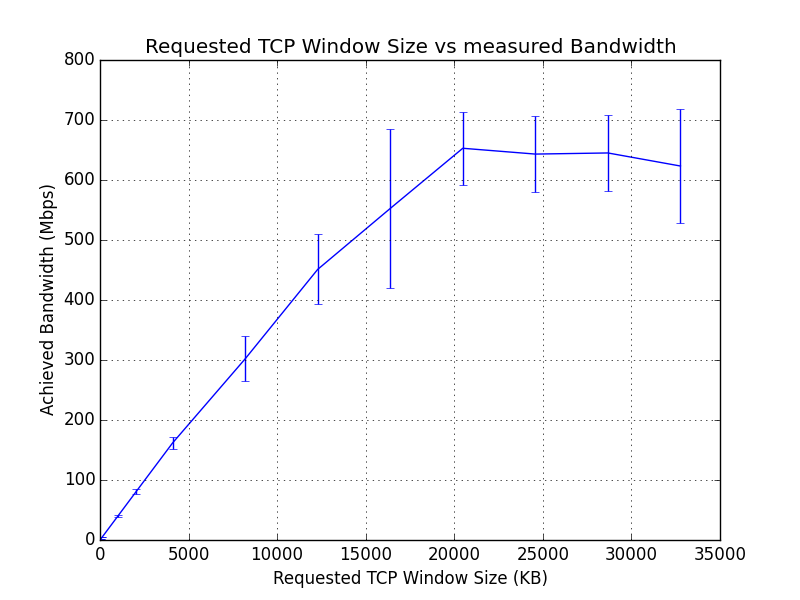
\includegraphics[width=0.5\textwidth]{img/iperf_vs_TCPws.png} \label{fig:iperf_a} }
\subfloat[]{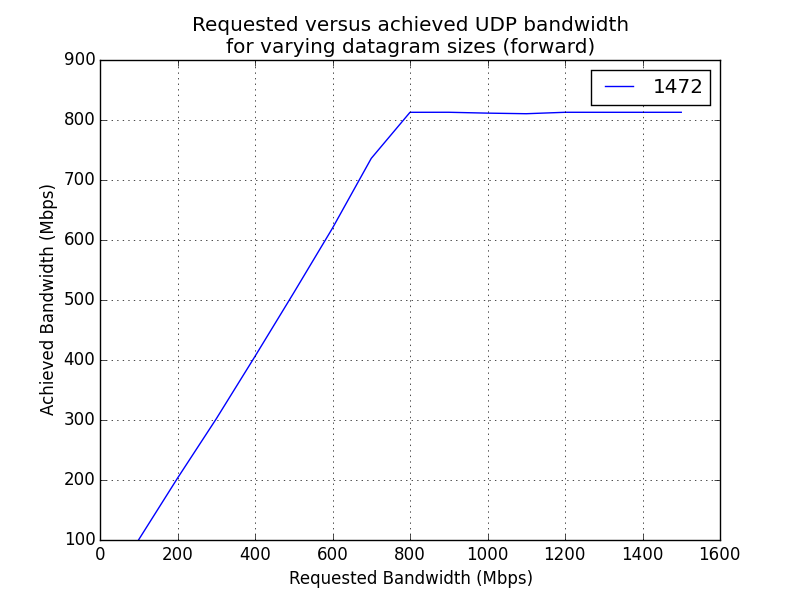
\includegraphics[width=0.5\textwidth]{img/iperf_vs_dsize_bw.png} \label{fig:iperf_b} }
}
\caption[]
% inserire samples: 600s -i 30s
{ TCP and UDT bandwidth measured by iperf scripts. Please note that the plot in (a) tends to present statistical fluctuations due to the load of the network,
this measure was performed during the night time on RFX side. }
\label{fig:iprf}
\end{figure}


\section{ Optimal segment size vs protocol }

The MDSplus connection is used to transfer experimental signals or parse evaluations and must be obviously reliable.
The transmission content is here represented by Signal Segments objects (segments hereafter). 
Segments are MDSplus objects that were designed to cluster signals in many shorter fragments and they are particularly suited to be network handled.
Tests has been performed using TCP and UDT, the latter based on UDP. 
~
The software can be set to send many parallel streams of segments each collected into a single signal at the target server.
We shall call these the connection channels and they are at most uncorrelated each others. The sole correlation resides on mdsip mutexes accessing parse files.
In the figures below the total speed reached by those channels is plotted against the per segment size for both protocols.

The Figure~(\ref{fig:sizea}) presents results for up to 8 TCP channels. 
For these TCP channels the Round Trip Time dominates the connection and MDSip performs far below the network capacity due to the fact that all sent packet from a MDSip client must be acknowledged by the MDSip server side at application layer, and this produce a double RTT delay when the segment size equals the TCP window.
The maximum throughput is reached aggregating channels of 40 KB segment size.
The overall connection speed is very poor and does not scale with different TCP windows sizes at all.
The main reason must reside in the \emph{mdsip} data checksumming mechanism application level and should be further investigated.
In any case the TCP seems to be very sensible to the network delay and appears to be non feasible for long distance connections.

On the other hand the UDT is a reliable UDP based application level data transport protocol designed for data intensive applications over wide area high-speed networks. 
It transfers bulks of data with its own reliability control and congestion control mechanisms achieving a much higher speed than TCP in such connections.
~
The results of UDT bandwidth is plotted in Figure~(\ref{fig:sizeb}).
This protocol appears very effective in this case gaining higher speed rates than the observed TCP iperf limit.

\begin{figure}[ht]
\centerline{
\subfloat[]{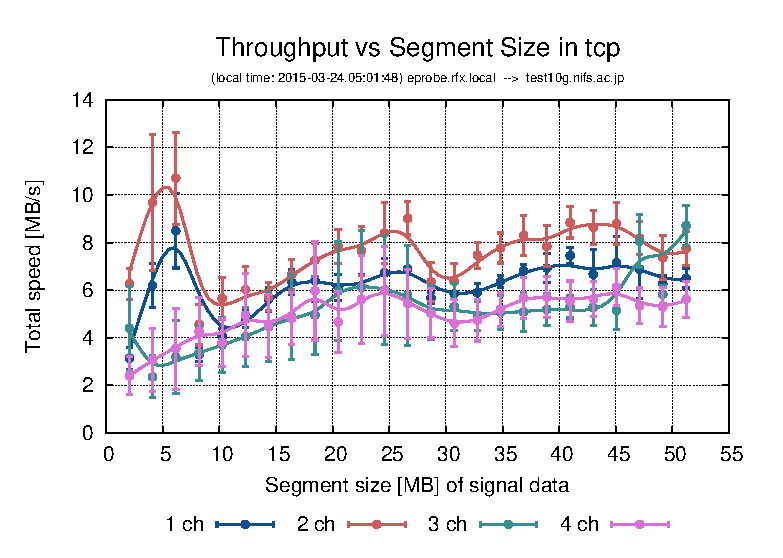
\includegraphics[width=0.5\textwidth]{img/size-tcp.eps} \label{fig:sizea} }
\subfloat[]{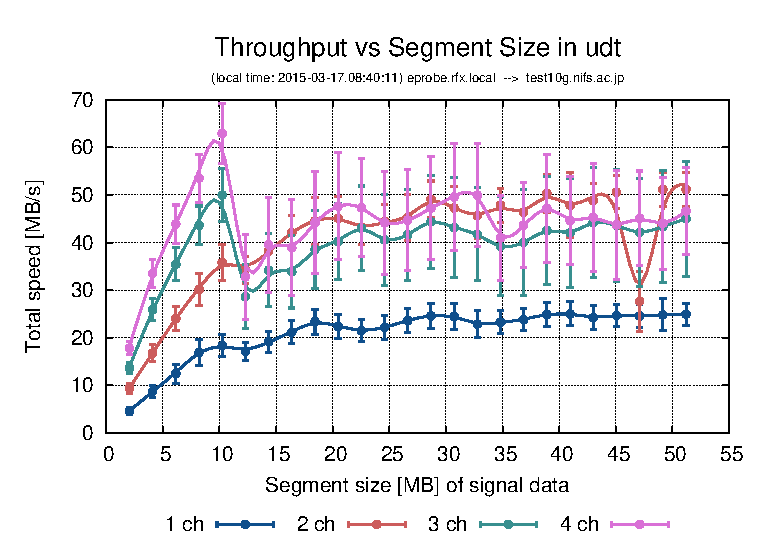
\includegraphics[width=0.5\textwidth]{img/size-udt.eps} \label{fig:sizeb} }
}
\caption[]
{ TCP vs UDT connection throughput }
\label{fig:size}
\end{figure}

The reliability of transported data is done by UDT at ISO/OSI application layer before making real data segment available to \emph{mdsip} optimizing the transfer, but the segment send operation is still acknowledged by \emph{mdsip} return statement producing a rising speed curve as the segments become larger.
Moreover the channel aggregation may ease this effect also increasing the overall speed where small segments must be sent.
But, as shown in figure, the augmented congestion penalizes this behaviour for more than two channels and we can conclude that the optimal number of parallel UDT streams should be left less than three for large bulk transfers.

Timings histograms are collected for each separate channel and added together in Figure~(\ref{fig:distr-tcp}) for TCP and in Figure~(\ref{fig:distr-udt}) for UDT.
In Figure~(\ref{fig:distr-tcp}) the 40 KB segment window timing distribution is plotted from set of 300 samples for two configurations, one channel transfer in blue line and aggregated eight channels in red.
Separated populations are clearly visible positioned at multiples of the 300 ms RTT.
~
\begin{figure}[ht]
\centerline{
\subfloat[]{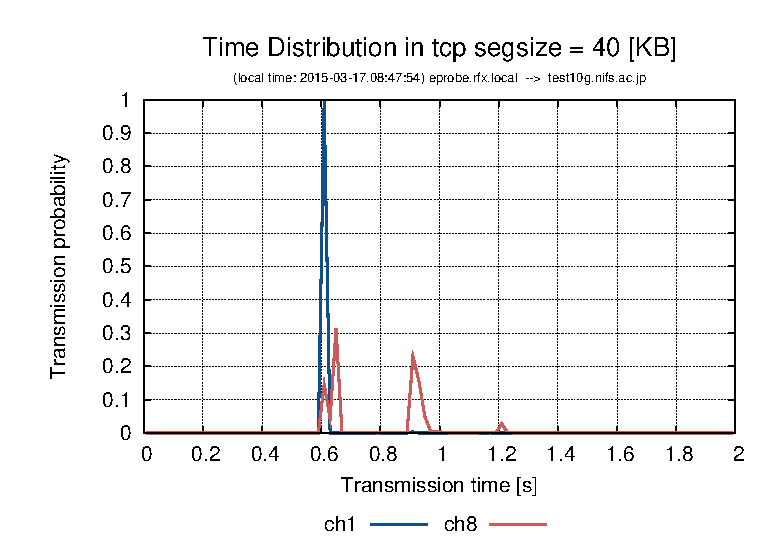
\includegraphics[width=0.5\textwidth]{img/distr-tcp-time.eps} \label{fig:fig1} }
\subfloat[]{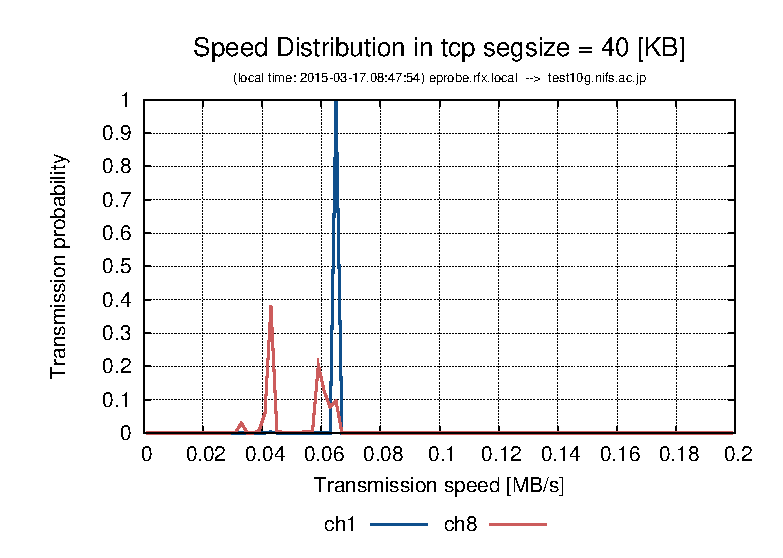
\includegraphics[width=0.5\textwidth]{img/distr-tcp-speed.eps} \label{fig:fig1} }
}
\caption[]
{ Timing distributions for TCP connection }
\label{fig:distr-tcp}
\end{figure}

For UDT connection the transmission times appears more spread.
Two populations emerge from the background separated by a single RTT, this probably shows the UDT request for retransmission of lost UDP datagrams.
When we have two channels or more the congestion handling masks these recurring values further spreading the times plot.
Finally the maximum achieved speed for 20 MB segment size is about 180~Mbps for single channel and 400~Mbps for two channels, this is not up to par with the assigned maximum bandwidth of the network but a good result for a reliable data transfer anyway.

\begin{figure}[ht]
\centerline{
\subfloat[]{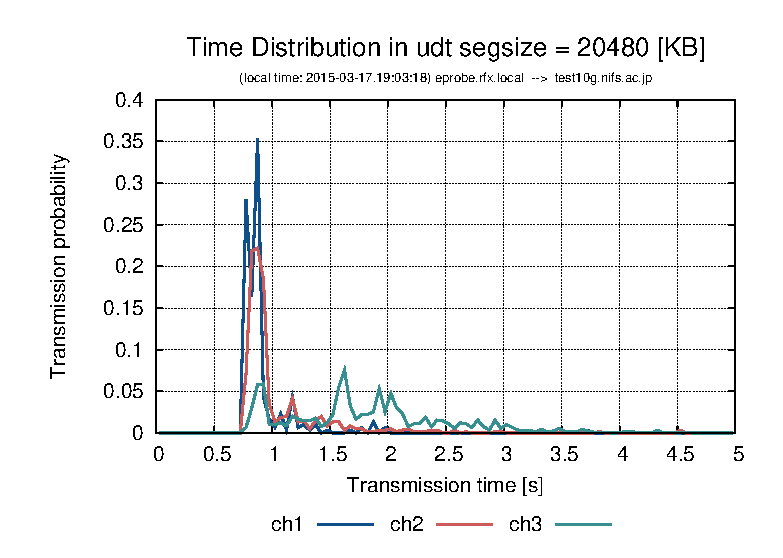
\includegraphics[width=0.5\textwidth]{img/distr-udt-time.eps} \label{fig:fig1} }
\subfloat[]{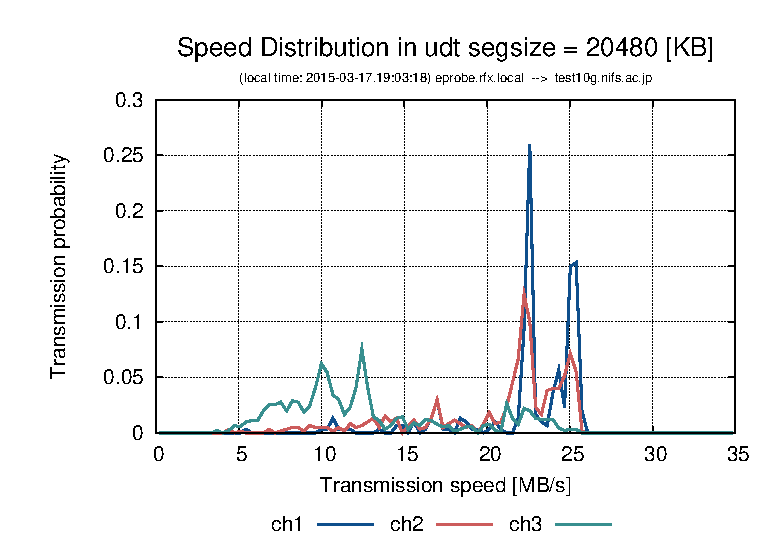
\includegraphics[width=0.5\textwidth]{img/distr-udt-speed.eps} \label{fig:fig1} }
}
\caption[]
{ Timing distributions for UDT connection }
\label{fig:distr-udt}
\end{figure}

\section{Transmitted Content}

Different generators of transmitted content were implemented to check for a possible content dependent behaviour of the network.
\emph{mdsip} was set to the maximum compression level that is also the default setting ("-c 9" command line argument).
Three signals were applied: a simple sine function of 6.28 [s] period and sampled in milliseconds, a white noise in the interval $(0,1)$ and a random variable from a normal distribution with zero mean and $\sigma=1$.
The throughput for the three signals (respectively labelled: \emph{sine}, \emph{noiseW} and \emph{noiseG}) are plotted against the segment size for a single channel connection for TCP Figure~(\ref{fig:content-tcp}) and for UDT in Figure~(\ref{fig:content-udt}).
There seems to be no evidence of any difference in transfer speed for the three cases reported so we can presume that a content dependency is not present within this network path and that \emph{mdsip} does not add a significant compression of these data sequences. Some test were also performed with a real case of a read RFX pulse, they show similar results that are not reported here\footnote{the \emph{eprobe} server is not allowed to access the RFX data files as it resides outside the firewall protected zone, so that this analysis is not possible at the moment}.

\begin{figure}[ht]
\centerline{
\subfloat[]{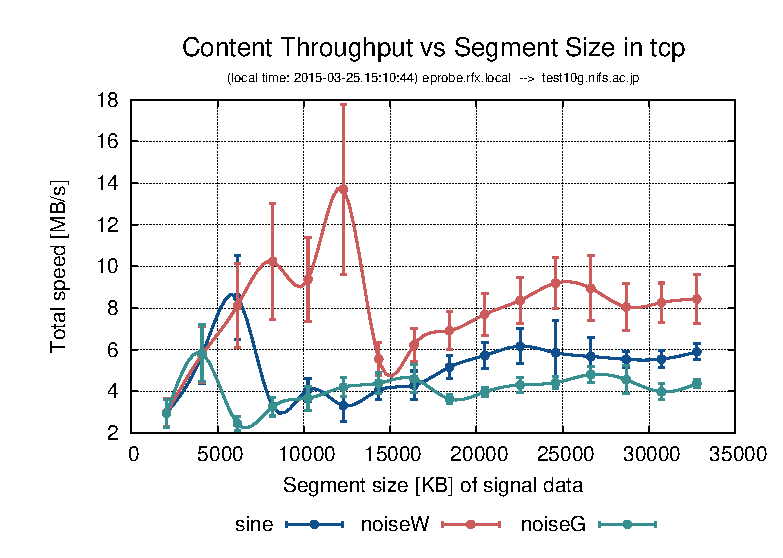
\includegraphics[width=0.5\textwidth]{img/content-tcp.eps} \label{fig:content-tcp} }
\subfloat[]{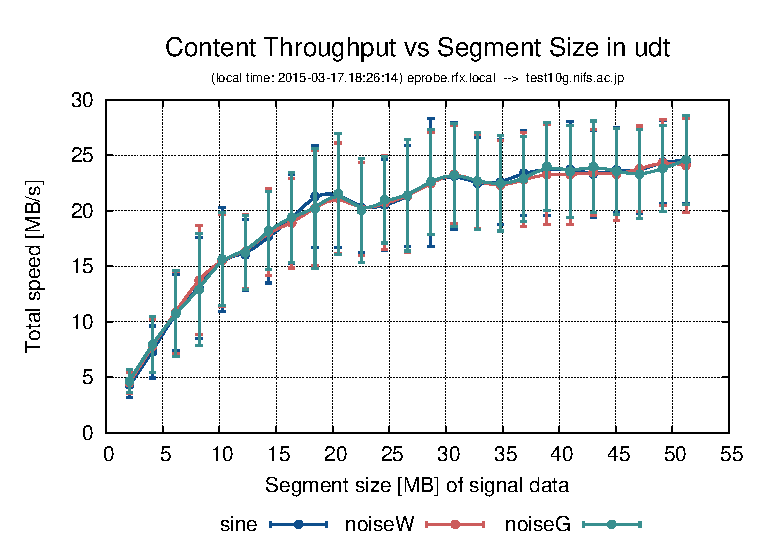
\includegraphics[width=0.5\textwidth]{img/content-udt.eps} \label{fig:content-udt} }
}
\caption[]
{ Single channel throughput versus transmitted segment size in TCP and UDT for three different content generators: sine, white noise and gaussian noise }
\label{fig:content}
\end{figure}



\section{Conclusions}

The long distance \emph{mdsip} internet link from Italy to Japan has been tested using a new ad-hoc test tool.
A preliminary tweak of the network connection has been done using iperf test results for the given endpoints.
Tests have been performed to find the best segment size and the optimal channels parallelization for the TCP and UDT transport protocols.
As expected the main result is that the UDT transport should be preferred to TCP in such fast long distance connections.

In any case the \emph{mdsip} TCP handling does not show to scale with any adjusting of TCP buffer size so there probably may be an improvement by this side.
% But, as the iperf tests reported, the achievable bandwidth for TCP will not over take the maximum value obtained using UDT so, for this particular case, we can foresee that any TCP tuning will not improve this result.
Moreover both protocols suffer the large RTT value of this link, this is much evident for small transmitted segments where the use of multiple parallel connections may be effective.
Once UDT is taken as the best transport, two independent channels shown to perform uniformly better than the single channel, but higher values must be used with care of the network congestion and should be used where the size of segments is mandatory small.

The network link and the \emph{mdsip} itself seems to be opaque to the nature of data to be transported as it shows no speed differences among three tested signal waveforms.

Finally the overall datum that can be extracted from this 1~Gbps internet link analysis is that the maximum achievable bandwidth of actual transported information is near to 50~MBps.
So that, with a proper tuning of the transported signals, the use of MDSplus for long distance sharing of fusion data can be a valuable choice.


\end{document}





